\documentclass[twoside,twocolumn]{article}

\usepackage{blindtext} 
\usepackage{graphicx}
\usepackage[sc]{mathpazo} 
\usepackage[T1]{fontenc} 
\linespread{1.05} 
\usepackage{microtype} 
\usepackage{multirow}


\usepackage[english]{babel} 


\usepackage[hmarginratio=1:1,top=32mm,columnsep=20pt]{geometry} 
\usepackage[hang, small,labelfont=bf,up,textfont=it,up]{caption} 
\usepackage{booktabs} 


\usepackage{lettrine} 


\usepackage{enumitem} 
\setlist[itemize]{noitemsep} 


\usepackage{abstract} 
\renewcommand{\abstractnamefont}{\normalfont\bfseries} 
\renewcommand{\abstracttextfont}{\normalfont\small\itshape} 


\usepackage{titlesec} 
\renewcommand\thesection{\Roman{section}} % 
\renewcommand\thesubsection{\roman{subsection}} 
\titleformat{\section}[block]{\large\scshape\centering}{\thesection.}{1em}{} 
\titleformat{\subsection}[block]{\large}{\thesubsection.}{1em}{} 


\usepackage{fancyhdr} 
\pagestyle{fancy} 
\fancyhead{} 
\fancyfoot{} 
\fancyhead[C]{Modelo Dimensional vs Modelo Tabular $\bullet$ Octubre 2019 $\bullet$ } 
\fancyfoot[RO,LE]{\thepage} 


\usepackage{titling} 


\usepackage{hyperref} 


%----------------------------------------------------------------------------------------
%	TILULOS
%----------------------------------------------------------------------------------------


\setlength{\droptitle}{-4\baselineskip} 

\pretitle{\begin{center}\Huge\bfseries} 
\posttitle{\end{center}} 
\title{Modelo Dimensional vs Modelo Tabular} 
\author{Jose  Luis Condori Choquecota\\
}
\date{Octubre 2019} 
\renewcommand{\maketitlehookd}{

\begin{abstract}
\noindent 
Desde el siglo pasado se ha investigado en aras de incrementar la eficiencia en el almacenamiento y el acceso a las bases de datos analíticas, sobre cuyos resultados las grandes compañías han introducido productos comerciales. En este escenario, Microsoft SQL Server 2012 ofrece dos opciones independientes para la creación de los modelos analíticos, el modelo multidimensional y el reciente modelo tabular. El presente trabajo profundiza en las características y potencialidades de cada uno, proponiendo los criterios más importantes que, a juicio de los autores, se deben tener en cuenta al emprender un nuevo proyecto. El modelo tabular utiliza técnicas de bases de datos en memoria y almacenamiento columnar, con algoritmos de compresión avanzados, lo que lo convierte en una alternativa muy eficiente y atractiva en algunos contextos.


\end{abstract}


\begin{abstract}
\noindent 
Since the last century, research has been carried out to increase storage efficiency and access to analytical databases, on whose results large companies have introduced commercial products. In this scenario, Microsoft SQL Server 2012 offers two independent options for the creation of analytical models, the multidimensional model and the recent tabular model. This work deepens the characteristics and potential of each one, proposing the most important criteria that, in the authors' opinion, should be taken into account when undertaking a new project. The tabular model uses database techniques in memory and columnar storage, with advanced compression algorithms, which makes it a very efficient and attractive alternative in some contexts.
\end{abstract}
}

%----------------------------------------------------------------------------------------

\begin{document}

% Print the title
\maketitle

%----------------------------------------------------------------------------------------
%	INTRODUCCION
%----------------------------------------------------------------------------------------

\section{Introduccion}
\lettrine[nindent=0em,lines=3]{A}ntes de comenzar cualquier proyecto de Business Intelligence (BI) con SQL Services Analysis Services (SSAS), debe abordar la cuestión de si usar un modelo tabular o multidimensional para su capa semántica de BI. Aunque el modelo tabular es la más reciente de las dos tecnologías, Microsoft dijo que el tabular no es un reemplazo para el modelo multidimensional.

Ofrecer dos tecnologías diferentes para crear la misma capa de BI crea mucha confusión para todos los desarrolladores diferentes por igual. La elección de usar un modelo tabular o multidimensional es una decisión múltiple, especialmente cuando necesita tomar esta decisión cuando los requisitos del proyecto aún están en pañales. Esta guía te ayudará a desentrañar la confusión.

Dicho esto, la tecnología detrás del modelo multidimensional es más madura y tiene muchas más características que ofrecer que la de la tabla. Por lo tanto, si necesita alguna función que el multidimensional le ofrezca a la tabla, no le gusta la reescritura (para obtener más funciones, consulte la documentación de Microsoft), ya sabe cuál elegir.




%----------------------------------------------------------------------------------------
%	Objetivos
%----------------------------------------------------------------------------------------


\section{Objetivos}

\begin{itemize}

\item \textbf{ Modelo Dimensional vs Modelo Tabularl}
\\
\item Comprender las bases sobre el analisis de los modelos dimensionales y tabulares
\item Desarrollar de cada uno de los diagramas existentes en los modelos y su objetivo especifico
\item Analizar los dos modelos que se plantean.
\\



\end{itemize}


%----------------------------------------------------------------------------------------
%	Marco teorico
%----------------------------------------------------------------------------------------


\section{Marco teorico}
\begin{enumerate}
\item \textbf{E} l modelo de datos dimensional, como ya se comentó en artículos anteriores, conlleva una técnica de modelado que facilita la compresión de la base de datos, haciéndola intuitiva para usuarios no expertos, y es comúnmente utilizada para implementar los DWH o DM.
Esta técnica goza de una gran aceptación y, a menudo, es elegida como la preferida para representar datos analíticos por cumplir simultáneamente con los siguientes requerimientos:\\ \\
\begin{itemize}
\item Dispone y estructura los datos de manera comprensibles para el usuario de negocio
\item Genera un alto rendimiento en las búsquedas desde la capa de reporting
\end{itemize}

Dentro del modelado de datos dimensional destacan 2 conceptos clave: hechos y dimensiones.

\begin{itemize}
\item\textbf{Hechos:} Son las métricas, normalmente valores cuantitativos (numéricos) susceptibles de ser agregados
\item \textbf{Dimensiones:} Son los valores cualitativos. Proporcionan descripciones a los hechos, aportando un contexto a los mismos.
\end{itemize}

Existen 2 técnicas para llevar acabo el modelado dimensional: el esquema de estrella y el esquema de copo de nieve.

\begin{itemize}
\item\textbf{Esquema de Estrella}
Un esquema de estrella es un modelo de datos formado por una tabla de hechos, que contiene los datos para el análisis, rodeada de las tablas de dimensiones.
Como podemos observar en la imagen 1 la tabla de hechos es TH-Ventas y está rodeada de las dimensiones TD-Almacén, TD-Producto y TD-Cliente, almacenando el ID de cada dimensión en la tabla de Hechos para, así, poder relacionar los atributos descriptivos de cada dimensión con la fila de la tabla de hechos.
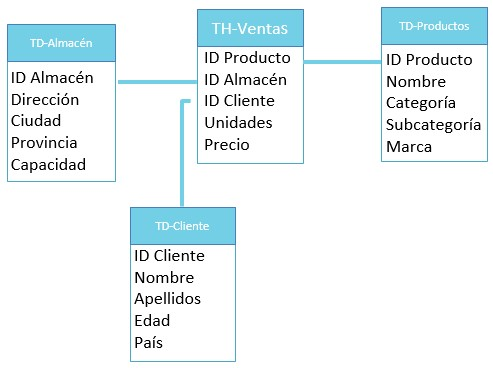
\includegraphics[width=7cm]{Imagenes/1.jpg}

El modelo estrella separa los datos del proceso de negocio en: hechos y dimensiones. Los hechos contienen datos medibles, cuantitativos, y las dimensiones los atributos que describen los datos indicados en los hechos.
\\\\

\item Tabla de hechos
\\
\item Clave principal compuesta por los claves principales de las tablas de dimensiones

\item Registra medidas o métricas de un evento específico. Ejemplo: cliente compra un geranio de maceta de 25cm en floristería mineral vegetal Lola a las 12:3 0am del 10 de Octubre de 2027

\item Evita repetir de manera completa los atributos dimensionales. En la TH sólo irá un ID de la dimensión

\item Se diseñan según el nivel de granularidad deseado, pudiendo registrar eventos a un gran nivel de atomicidad
\\\\
\item Tabla de dimensiones\\
Tienen una clave primaria simple.
\\

\item Generalmente tienen un número bajo de registros
\item Cada registro puede contener un gran número de atributos
\item Suelen contener una surrogate primary key, generalmente una columna de tipo entero


\item \textbf{Esquema en Copo de Nieve:} 
Es una estructura más compleja que el esquema de estrella. Se da cuando alguna de las dimensiones se implementa con más de una tabla de datos.
El objetivo es normalizar estas tablas y reducir el espacio de almacenamiento al eliminar la redundancia.
Se representa como una tabla de hechos conectada con dimensiones anidadas. Al normalizar por completo las dimensiones el resultado parece un copo de nieve.
\end{itemize}
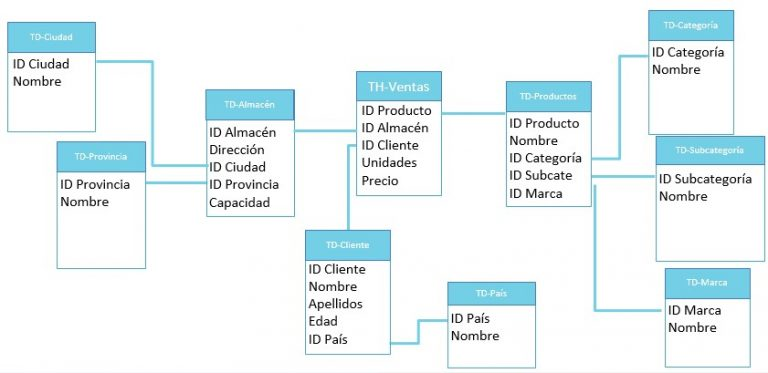
\includegraphics[width=7cm]{Imagenes/2.jpg}
\textbf{ {\small}}
\\ \\

Observamos en la imagen 2 como se dividen las dimensiones de TD-Almacén, TD-Producto y TD-Cliente en sub-dimensiones normalizadas.\\


\textbf{Las principales ventajas del esquema de copo de nieve son}
\begin{itemize}
\item Algunas herramientas de modelado de bases de datos multidimensional OLAP se optimizan
\item La normalización de los atributos reduce el almacenamiento de datos
\end{itemize}
\textbf{Las principales desventajas del esquema de copo de nieve son:}
\begin{itemize}
\item Queries complejas debido a la normalización (implica un mayor número de cruces)
\item Bajo rendimiento debido a la normalización
\end{itemize}


   
\textbf Modelo Tabular \\ 


Todos los que hayan trabajado en Business Intelligence con las herramientas de Microsoft ya conocen lo que son los proyectos Multidimensionales de bases de datos. Son bases de datos hechas para la generación de reportes con un diseño especial muy diferente a las bases de datos transaccionales y con otro motor de base de datos.

Los modelos tabulares son bases de datos “en memoria” de Analysis Services. Gracias a los algoritmos de compresión avanzados y al procesador de consultas multiproceso, el motor analítico en memoria xVelocity (VertiPaq) ofrece un acceso rápido a los objetos y los datos de los modelos tabulares para aplicaciones cliente de reportes como Microsoft Excel y Microsoft Power View.

Los modelos tabulares admiten el acceso a los datos mediante dos modos: modo de almacenamiento en caché y modo DirectQuery. En el modo de almacenamiento en caché, puede integrar datos de varios orígenes como bases de datos relacionales, fuentes de distribución de datos y archivos de texto planos. En el modo DirectQuery, puede omitir el modelo en memoria, lo que permite a las aplicaciones cliente consultar los datos directamente en el origen relacional (SQL Server).
Analysis Services proporciona funciones de procesamiento analítico en línea (OLAP) y minería de datos para aplicaciones de Business Intelligence.

Los proyectos multidimensionales si bien les falta mucho para poder ser tan estables como las bases de datos transaccionales, están en una etapa más avanzada de desarrollo y grandes empresas ya lo utilizan.


\begin{enumerate}
\item[1] Ventajas del modelo tabular:\\ 
\item Mucho más veloz en consultas.
\item No requiere generar Aggregations (agregaciones) por lo que se simplifica el tiempo de procesamiento.
\item Gracias al DAX (el lenguaje para acceder a los datos equivalente al MDX), tiene mayor flexibilidad para obtener información.
\item Es intuitivo por lo que es mucho más rápido y fácil de entender e implementar.
\item Se basa en modelos relacionales.\\ \\ 


\item[2] Problemas con el modelo tabular: \\ 
\item[(a)] Las particiones no se procesaban en paralelo si no secuencialmente, lo que hace que sea más lento el procesamiento.
\item[(b)]No se pueden usar multiples idiomas.
\item[(c)]Si son muchos datos tarda bastante en manejar configuraciones de diferentes particiones.
\item[(d)]El modelo tabular acapara demasiada memoria RAM y a su vez es dependiente de tal que afectará a otras aplicaciones.

\item[2] Ventajas del modelo multidimensional: \\ 
\item[(a)]La razón principal para generar un modelo multidimensional de Analysis Services es lograr el rendimiento rápido de consultas ad hoc en los datos empresariales. Un modelo multidimensional se compone de cubos y dimensiones que se pueden anotar y ampliar para admitir construcciones de consultas complejas. Los desarrolladores de BI crean cubos para obtener tiempos de respuesta rápidos y para proporcionar un único origen de datos para reportes empresariales.

Debido a la mayor importancia de business intelligence en todos los niveles de una organización, el hecho de tener un solo origen de datos analíticos se garantiza que las discrepancias se mantienen al mínimo, si no, se eliminan por completo.
\item[(b)]Otra ventaja importante del uso de las bases de datos multidimensionales de Analysis Services es la integración con las herramientas de informes BI utilizadas habitualmente, como Excel, Reporting Services y PerformancePoint, así como las aplicaciones personalizadas y las soluciones de terceros.




\end{enumerate}
    
\end{enumerate}





%----------------------------------------------------------------------------------------
%	Ejemplo
%----------------------------------------------------------------------------------------



%----------------------------------------------------------------------------------------
%	Análisis
%----------------------------------------------------------------------------------------


\section{Análisis}
Tabular mode tiene algunas ventajas sobre modelos multidimensionales pero también tiene algunas desventajas.:\\
\begin{itemize}
 \item El escenario consiste de una base de datos de 16.4 GB con una tabla de hechos con 100 millones de registros que tiene menos de 10 columnas. El comparativo al cargar ésta información tanto a Tabular Mode como a multidimensional se muestra a continuación:\\
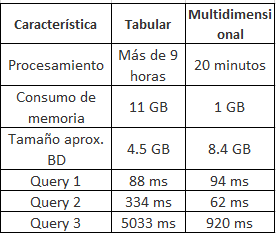
\includegraphics[width=7cm]{Imagenes/3.png}
\textbf{ {\small}}
\\ \\



\end{itemize} 



%----------------------------------------------------------------------------------------
%	CONCLUSIONES
%----------------------------------------------------------------------------------------

\section{Conclusiones}
\begin{itemize}	
 \item A la hora de definir nuestro modelo SSAS debemos analizar concienzudamente los diversos usos e implementaciones del que va a ser objeto el producto final, ya que aunque ambos tipos de elementos se creen en la herramienta de SSAS hay diferencias sustanciales, no que hagan que uno sea mejor y el otro peor si no que van encaminados a diferentes propósitos.

Una de la primeras y más importantes diferencias es que el motor de almacenamiento de los modelos tabulares es en memoria y persiste en disco, lo que garantiza su recuperación tras un reinicio.

Además su arquitectura permite que se generen modelos rápidamente ya que su implementación es sencilla y permite performance de rendimiento.

Los modelos tabulares están basados en columnas y no existe el concepto de agregaciones, lo que quiere decir, que cuando se realicen consultas sobre el mismo el motor de consulta solo trabajará con las columnas que figuren en la consulta.

Por último, en tabular no existe el concepto de “agregaciones” que existe en los cubos multidimensionales. El almacenamiento en los modelos tabulares está basado en columnas, esto es, que cuando se realiza una consulta MDX, el motor de consulta solo trabajará sobre las columnas especificadas en la consulta.

Por otro lado tienen limitaciones,como que es no se permite más de una relación entre dos tablas, no se permiten relaciones muchos a muchos entre dos tablas o que para extraer datos del origen es necesario realizarlo mediante una única consulta por cada tabla del modelo.
\\


\end{itemize} 



%----------------------------------------------------------------------------------------
%	BIBLIOGRAFIA
%----------------------------------------------------------------------------------------


\begin{thebibliography}{99} 

\bibitem[1]{}
\newblock http://msdn.microsoft.com/es-es/library/hh212945.aspx

\bibitem[2]{}
\newblock http://technet.microsoft.com/es-es/library/ms143708.aspx

\bibitem[3]{}
\newblock http://msdn.microsoft.com/es-es/library/hh230904.aspx

\bibitem[4]{}
\newblock https://geeks.ms/lmblanco/2019/07/22/ssas-tabular-ssis-y-power-bi-en-accion-modelo-tabular-diseno-y-carga-de-datos/
\bibitem[5]{}
\newblock https://amby.net/2018/02/13/dax-introduccion-a-las-relaciones-del-modelo-tabular/
\bibitem[6]{}
\newblock https://blog.bi-geek.com/modelo-dimensional/ 




\end{thebibliography}


%----------------------------------------------------------------------------------------


\end{document}
